\section{Symulacyjny model wymiennika}
Zadanie polegało na symulacji wymiennika energii cieplnej do sieci ciepłowniczej AGH. Należało pod wpływem zmian temperatury zasilania miejskiego generować odpowiednią wartość  temperatury wody w sieci AGH, tak aby zapewnić wystarczającą moc cieplną do utrzymania odpowiednich warunków w budynkach.
	\subsection{Opis algorytmu i realizacji zadania}
    Realizacja zadania rozpoczęła się od stworzenia modelu symulacyjnego w pakiecie \textit{Simulink} na podstawie równań otrzymanych w instrukcji (Rys. \ref{Wymiennik_Sim}).
    \begin{figure}[htb]
		\centerline{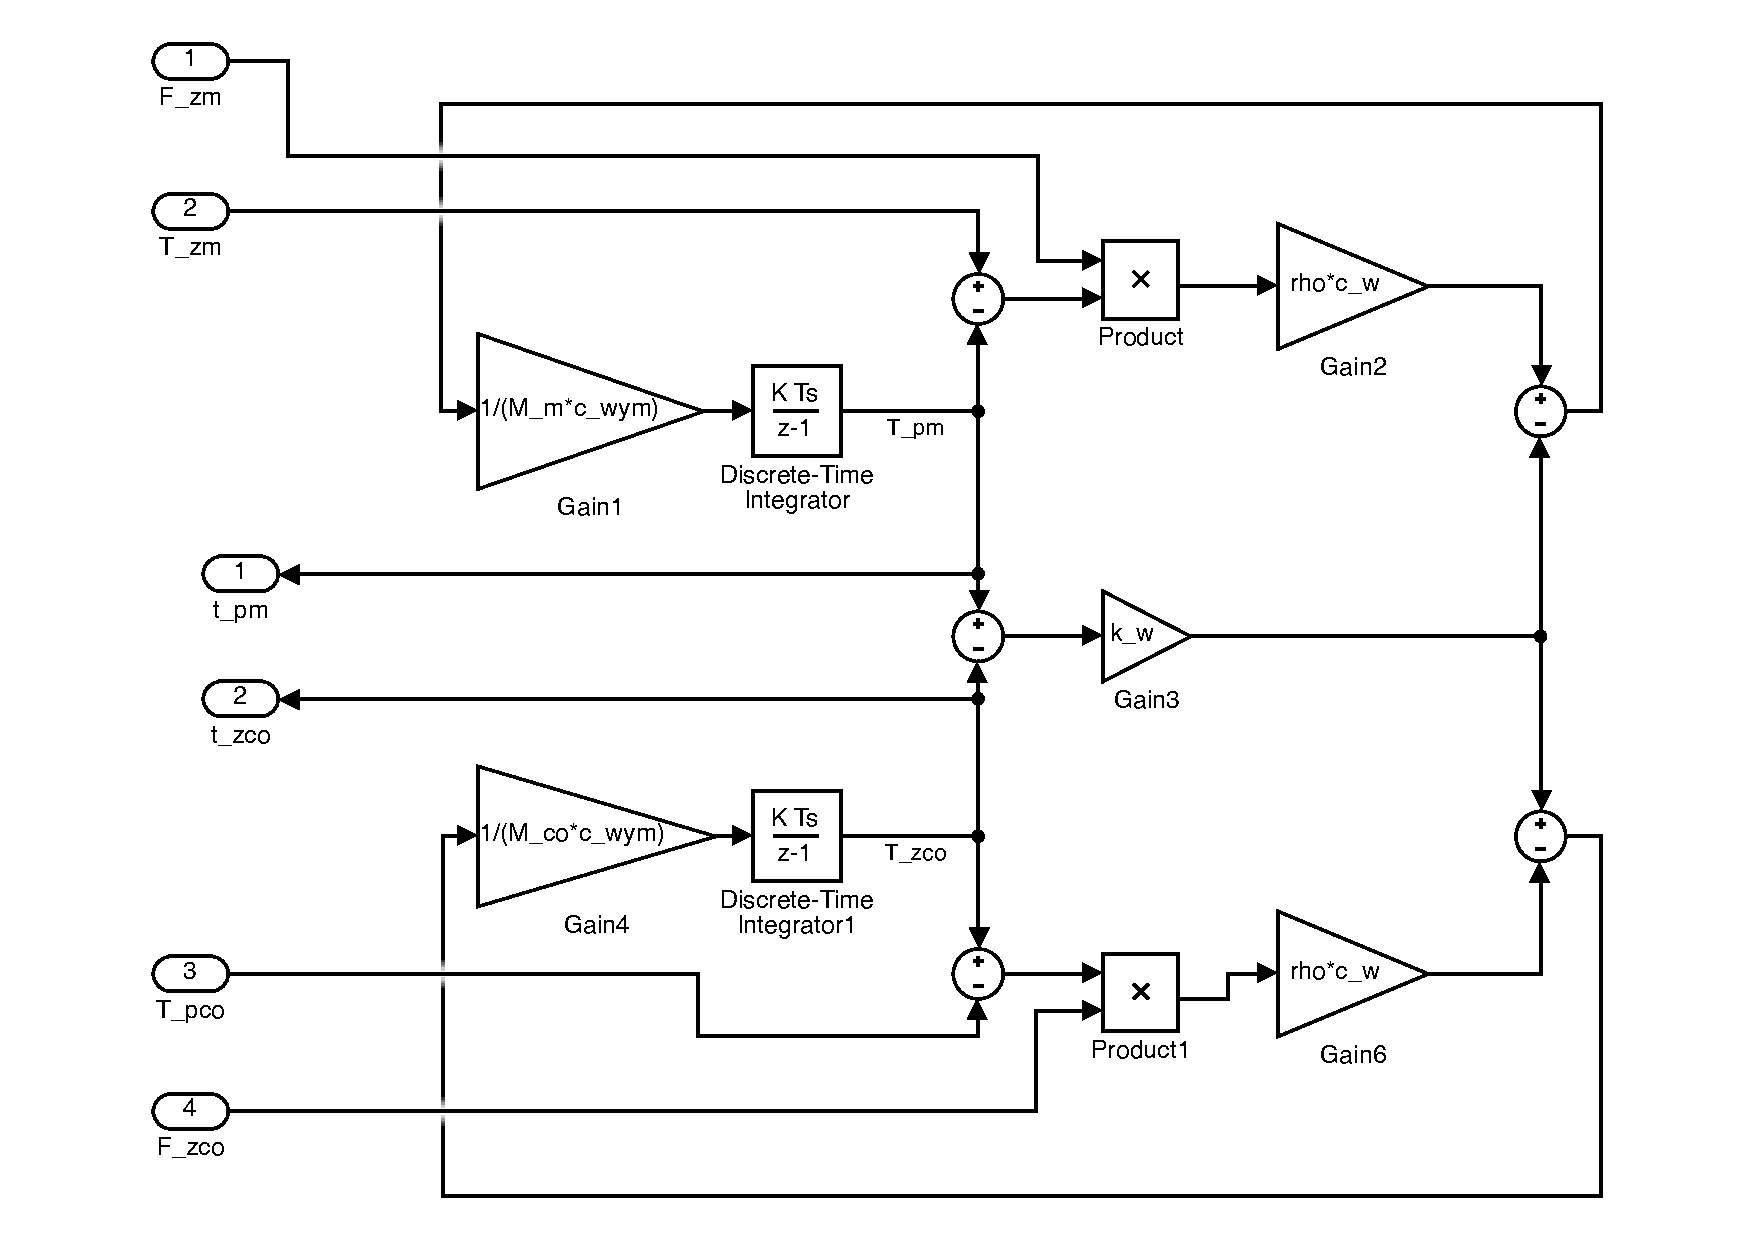
\includegraphics [width=0.8\textwidth,center] {Wymiennik_Sim.pdf}}
		\caption{Model symulacyjny wymiennika}
        \label{Wymiennik_Sim}
	\end{figure}
    Następnie z pomocą pakietu \textit{Embedded Coder} została wygenerowana aplikacja w języku C, której zadaniem była symulacja przebiegu temperatur. Przyjęty został krok próbkowania równy $0.5s$, co przy 60-krotnym przyspieszeniu czasu oznaczało 120 iteracji symulacji. Program został zmodyfikowany, by przyjmował czas symulacji jako argument startowy oraz zapisywał temperatury w pliku. Czas obliczeń dla 60 sekund symulacji jest niemożliwy do zmierzenia tradycyjnymi narzędziami. Dopiero symulacja czasu dwóch tygodni pozwoliła uzyskać $34ms$. Dzięki takiemu podejściu wykonywania obliczeń w zoptymalizowanej aplikacji poza serwerem MODBUS, uzyskane zostało znaczne przyspieszenie.
    
    Z powodu wykorzystania w komunikacji ograniczonej dokładności danych -- do 2 miejsca po przecinku, przeprowadzona symulacja całego układu nieznacznie odbiega od modelu quasi-ciągłego, różnicę dla rozgrzewania od temperatury $15^\circ C$ przy parametrach: 
    $$F_{zco} = 0.035, F_{zm} = 0.015, T_{zm} = 70^\circ C, T_{pco} = 50^\circ C$$
    przedstawia rysunek \ref{Wymiennik_CMP}. Jak widać nie jest ona znaczna biorąc pod uwagę stałe czasowe obiektu. Dla temperatury $t_{zco}$ maksymalna odchyłka wynosi $0.63^\circ C$, a dla $t_{pco}$ -- $0.45^\circ C$.
    \begin{figure}[htb!]
		\centerline{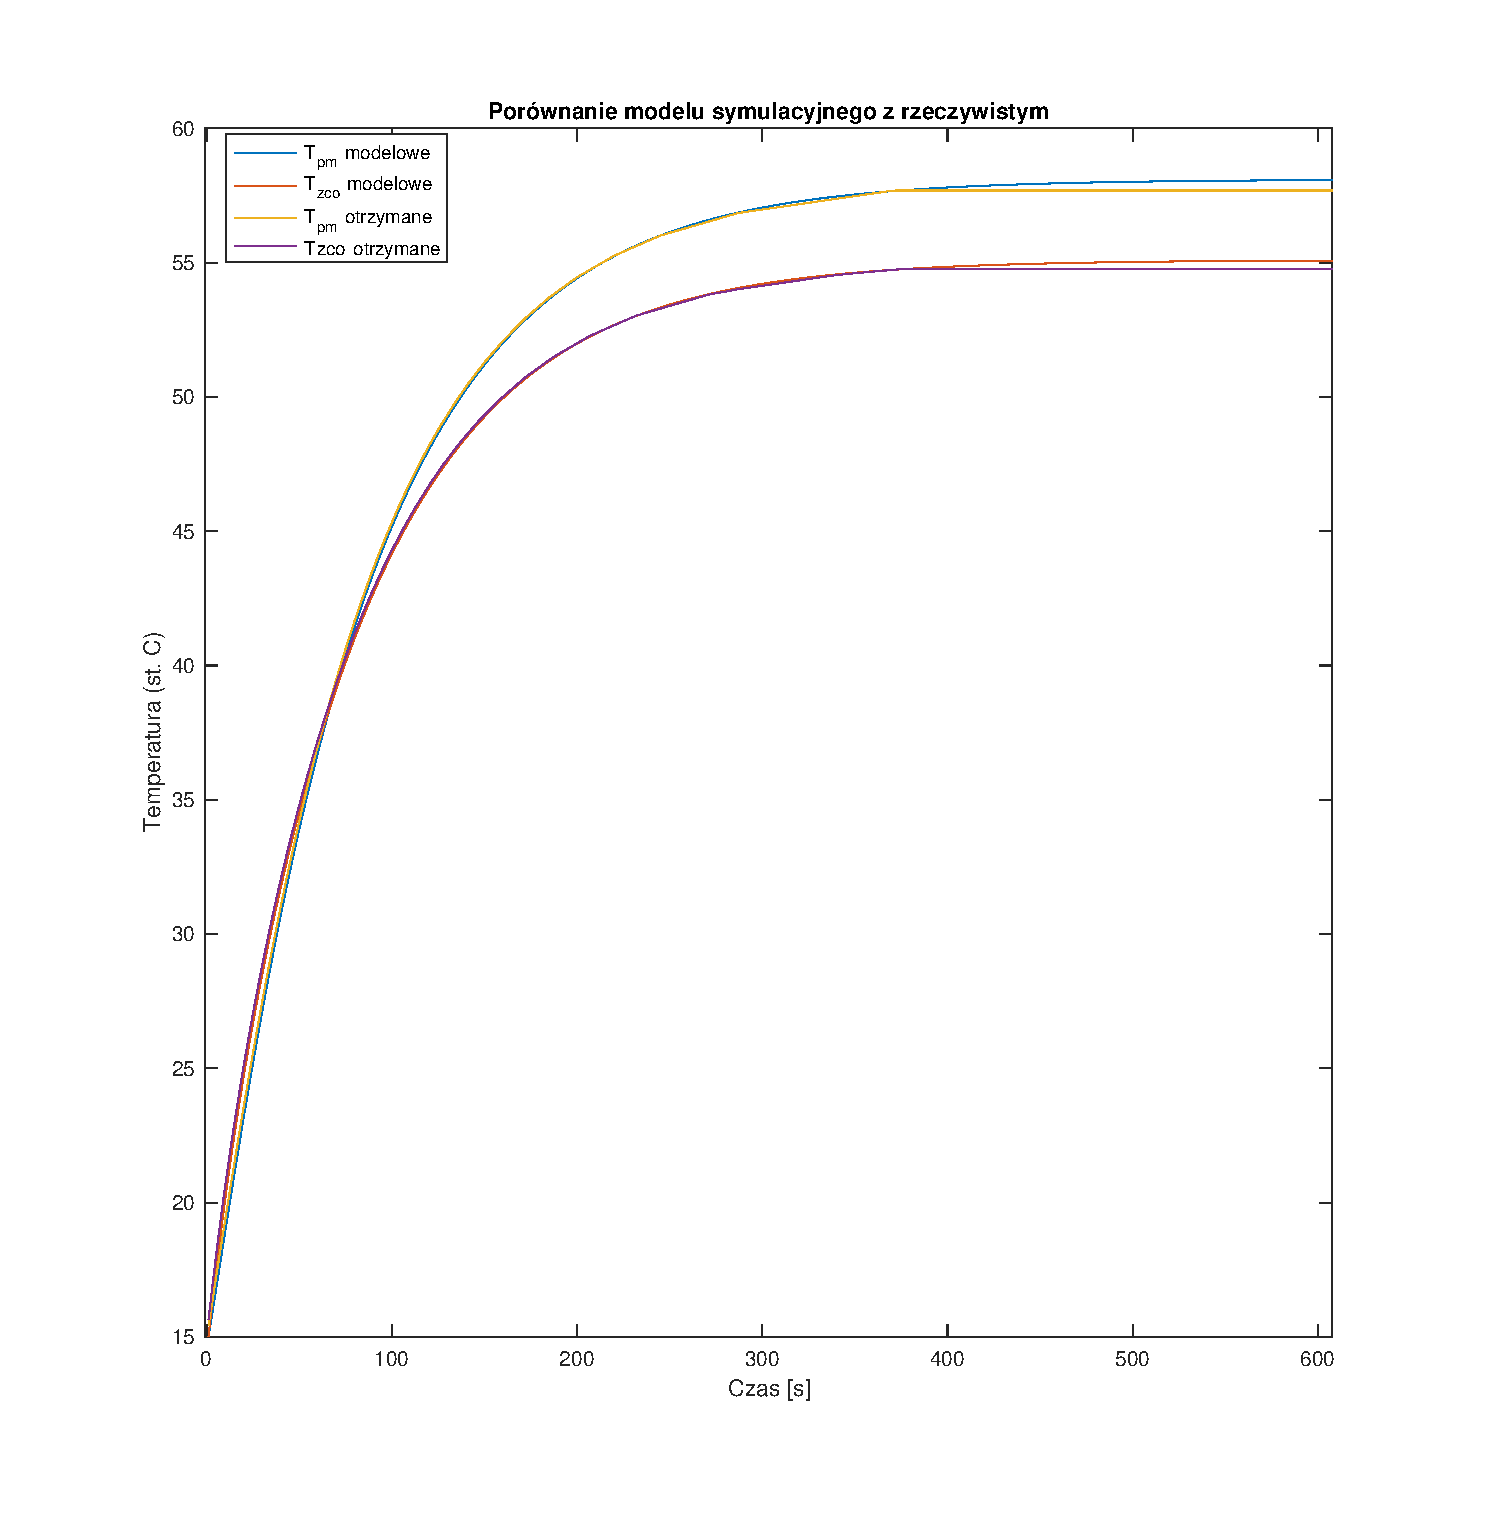
\includegraphics [width=0.8\textwidth,center] {wymiennik_cmp.eps}}
		\caption{Porównanie wyników dokładnego modelu oraz użytego w symulacji}
        \label{Wymiennik_CMP}
	\end{figure}
    
\subsection{Opis realizacji komunikacji sieciowej}    
    W celu komunikacji sieciowej użyto biblioteki PyModbus języka Python.
Struktura programu odpowiadającego za komunikację była dwuczęściowa. W głównym wątku wywołane były dwie funkcje dwóch różnych klas.

	Jeden obiekt pełnił rolę odbiorcy (klasa Server) zawierającego bloki rejestrów i cewki. Część odbiorcza pełniła dwie podstawowe funkcje:
	\begin{itemize}
	\item odczyt wartości wpisanych do rejestrów przez nadawców (zarówno wartości wielkości fizycznych do symulacji jak i aktualną wartość czas od dostawcy czasu)
	\item ustawienie flagi \textit{ready\_to\_send} dla części nadawczej, która informowała o prawidłowym odczycie wartości i możliwości wykonania symulacji oraz wysłania wartości do odbiorców
	\end{itemize}
	Inicjalizacja części odbiorczej polegała na zapewnieniu właściwego adresu IP oraz portu, a także zdefiniowaniu funkcji, która była wywoływana po każdej dostawie wartości czasu. Tą funkcją było ustawienie flagi \textit{ready\_to\_send}.
Serwer pracował cały czas w osobnym wątku, po wywołaniu przez część nadawczą udostępniał odebrane dane.

	Druga część programu (obiekt klasy Sender) miała następujące zadania:
	\begin{itemize}
	\item realizowała właściwą symulację pracy wymiennika
    \item wysyłanie odpowiednie wartości do zdefiniowanych odbiorców
    \item ustawienie flagi \textit{ready\_flag} dla części odbiorczej, która informowała o gotowości do ponownego odebrania wartości czasu
	\end{itemize}
    Po inicjalizacji obiektu oraz zdefiniowaniu listy odbiorców w postaci budynków, regulatora oraz loggera danych wywoływana była podstawowa funkcja odpowiedzialna za ciągły odbiór danych, symulację i wysyłanie.

	W pierwszej kolejności następował odczyt wartości z rejestrów części odbiorczej. Jeżeli odbiornik dodatkowo ustawił flagę \textit{ready\_to\_send}, wykonywana została symulacja dla okresu wyliczonego na podstawie dwóch ostatnich wartości czasu. Następnie funkcja iterowała po wszystkich zdefiniowanych odbiorcach wymiennika i jeśli odbiorca był połączony to zapisywała odpowiednią wartość w jego rejestrze.

	Kolejnym krokiem po wysłaniu wartości było anulowanie flagi \textit{ready\_to\_send}, co oznaczało oczekiwanie na otrzymanie nowych wartości od części odbiorczej. Niezależnie czy zostało zrealizowane wysyłanie, kolejnym krokiem było ustawienie flagi \textit{ready\_flag} dla części odbiorczej, czyli gotowość zgłaszaną symulatorowi upływającego czasu. Na końcu funkcja tworzyła nowy wątek dla niej samej, co pozwalało zachować ciągłość wykonywania operacji.

    \subsection{Podsumowanie i wnioski}
    Najbardziej wymagającym czasowo elementem algorytmu jest komunikacja z użyciem protokołu modbus. Czas potrzebny na zapis flag jest ściśle zależny od obciążenia w sieci i ze względu na komunikację z wieloma klientami, zdarzały się spowolnienia symulacji powodowane przez wymiennik - najczęściej było to oczekiwanie na zakończenie symulacji przez któryś z budynków. 
    
    Kod stworzonego serwera oraz aplikacji symulacyjnej znajduje się w repozytorium pod adresem: \url{https://github.com/collargol/HeatExchanger}.
